
\section{Ontology Usage}
\label{chap:usage}

% ontologie mohou dobre popsat openstack architekturu, protoze openstack vyuziva message bus, service catalog. Ontologie slouzi pak nad ramec openstack sluzeb u serveru ale definuji i vlastni operacni systemy a pridruzene sluzby - monitorting, metering, firewally, backupy, log management atd

The journey to mapping high level models in ontologies was long. It was a process of describing everchanging OpenStack cloud architectures over past 2 years. The OpenStack foundation has released 4 major versions with 12 minor versions over that period. The number of managed software components grew from 5 to 17. At the beginnings we started mapping meta-data models in separate files containing complete meta-data set of all services for each server or device. The meta-data was encoded in YAML format. This approach was fine at earlier versions of OpenStack we tested as just the basic set of OpenStack services existed at the time. 

\medskip

\noindent
{\it Simple meta-data in YAML format}
\begin{verbatim}
service_name:
  service_role:
    data_parameter1: data_value1
    data_parameter2: data_value2
    data_parameter3:
    - data_value3a
    - data_value3b    
    object_parameter:
     object1:
       data_parameter1a: 
\end{verbatim}
\noindent

The next step was storing the service meta-data in hierarchical databases. The meta-data was split into separate files. The final meta-data for given resources is assembled using the two simple methods. The deep merging of several service definition fragments and parameter interpolation where parameters can be referenced. The reclass \cite{Reclass} was used to implement the desired data manipulation behaviour.

\medskip

\noindent
{\it Meta-data in YAML format, parameter interpolation}
\begin{verbatim}
service_name:
  service_role:
    data_parameter1: data_value1
    data_parameter2: {service_name:service_role:data_paramer1}
    object_parameter:
     {otherobject:object1}
\end{verbatim}
\noindent

This was elegant solution that could easily model growing number of services, but still lacked mechanisms to validate given data or encapsulate semantics. It helped to determine the domain and scope of new ontology. The ontology should use existing standards and provide vocabulary to define OpenStack services, core services and later network and storage resources. The ontology should provide mechanisms to validate schema for integrity issues, as missing parameters, disjoint services or values out of proper value domain.

% ontologie je multitenantni podporuje vice reseni najednou

All OpenStack services can be very well described by ontology as they communicate over common message bus, serialize their state and expose services through interfaces in a same way. The resource within ontology have data properties that are derived mostly from Dublin Core metadata terms. Other extensively used standard is OCLS Configuration Management resource definitions and Service-Oriented Architecture Ontology.  Resources can have object property types that describe more complex relations. Following example shows excerpt from Glance image service definition on the the controller node: 

\medskip

\noindent
{\it Meta-data in OWL-DL format}
\begin{verbatim}
  <owl:Class rdf:about="#CinderVolumeService">
    <rdfs:subClassOf>
      <owl:Class rdf:about="#VolumeService"/>
    </rdfs:subClassOf>
    <owl:disjointWith>
      <owl:Class rdf:about="#"/>
    </owl:disjointWith>
    <owl:disjointWith>
      <owl:Class rdf:about="#NovaVolumeService"/>
    </owl:disjointWith>
  </owl:Class>
\end{verbatim}
\noindent

\subsection{Implementation details}

% Vytvorerin ontologie - protoege, na zaklade SOA ontologie
% testovani reasoningu pres pellet vyvozovani

Initial work on creating our Ontology was done in Protege, open-source ontology editor and framework for building intelligent systems. It took some time to evolve ontology classes and create necessary dictionaries \cite{OntologyEvolution} to cover first IaaS architectures. Figure \ref{fig:cm} shows the current ontology service architecture.

The ontology is transformed into graph database using our python-bases service named django-ENC that can read and write ontology from OWL-DL XML files created by Protege and communicates with neo4j graph database through REST API. The graph databases are part of family of NoSQL databases and offer much better performance at any volume of data.

\begin{figure}[!h]
\centering
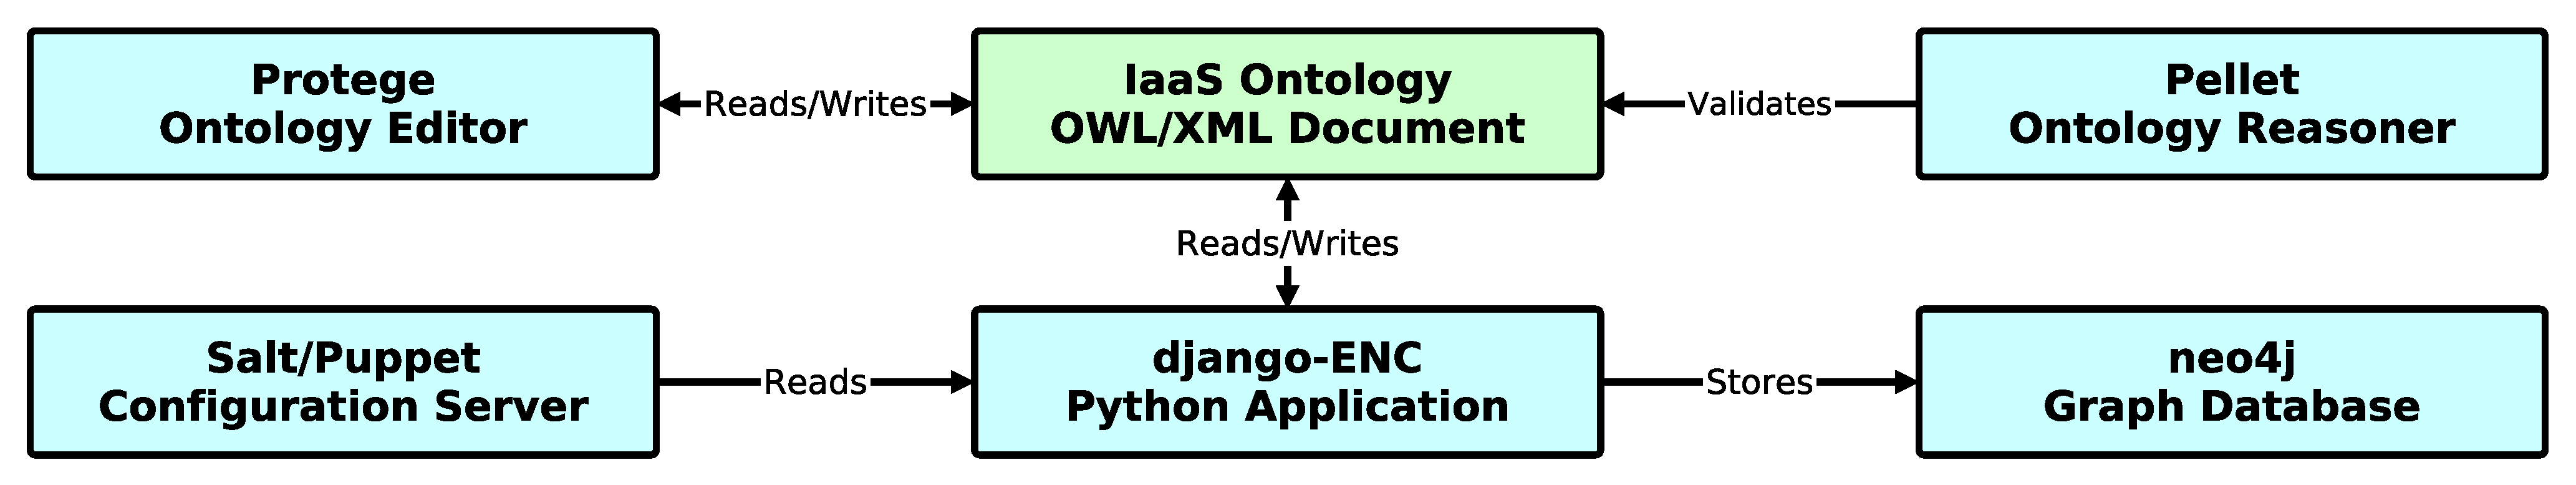
\includegraphics[scale=.17]{img/django_enc_arch.eps}
\caption{Ontology Service Architecture}
\label{fig:cm}
\end{figure}

The django-ENC service use web framework Django to provide web services and asynchronous task queue Celery to perform time consuming tasks like ontology assertions and synchronizations between XML and graph database. The HTTP REST API that can be consumed by configuration management tools like Salt or Puppet through their External Node Classification interface. The meta-data passed to configuration management tools is valid for level 1, 2 and 3 of unified cloud computing ontology \cite{OntologyComputing}. 

We have successfully tested service status enforcement of several complete OpenStack installations by SaltStack configuration management tool with meta-data acquired from Ontology Service API. The deployment process is not yet fully automated as there is need of setting up network and storage resources manually (only servers are provided), but the progress in both configuration management tools and network and storage will allow better automation of these components by in-place agents or access protocols like SSH in the future.

% \subsection{Model Architecture Sample}

% Given use case scenario Locality 2 we have 3 virtual servers providing OpenStack and other core services with 2 virtual servers providing SDN controllers in high-availability mode.

%\subsubsection{Common service components}

%All servers within archecture contain basic set of services necessary for long-term operation.

%linux.system, linux.network, linux.storage - Basic configuration of network interfaces, users, volume, mounts, etc.

% ntp.client - Time synchronisation accress all resources is important for correct communication incommon message bus

% salt.minion/pupper.agent - Configuration management clients enforce the model configuration to the actual servers.

%collectd.client, sensu.client - Monitoring services that provide common checks and meters for all services on the same server.

%\subsubsection{OpenStack Controller service components}

%OpenStack controller node provides core OpeStack services in 

%mysql.cluster, rabbitmq.cluster, haproxy.proxy, corosync.cluster - These services form the highly available foundation for the

%keystone.server, glance.server, nova.server, cinder.server, horizon.server - are services running on each controller providing capacity for load-balancing and disaster recovery.

%\subsubsection{SND Controller service components}

%SDN controller node controls the network resources.

%neutron.server, contrail.analytis, contrail.control, contrail.config - Configure

%\subsubsection{Compute node service components}

%Compute nodes hava the least services and these control the actual virtual server spawning.

%nova.compute, neutron.switch - These services control the actual virtualisation service, prepare the environment as networks and volumes for new servers and operate them.
